\documentclass[9pt, notes=hide]{beamer}

\usepackage[utf8]{inputenc}
\usepackage[spanish]{babel}
\usepackage{pgf}
\include{pythonlisting}

\setbeamertemplate{navigation symbols}{}
\usetheme{Warsaw}
\mode<presentation>
\title{Python Bytecode}
\subtitle{Python Behind the Scenes}
\author{Matías Bordese}
\institute{}
\logo{\pgfimage[width=0.5cm]{images/logo1}}
\date{PyCon Argentina\\Octubre de 2011}

% \newread \instream
% \def\DelimitedInclude#1#2{{
%     \openin \instream #1
% %     \read10 to \verbatim
%     \closein \instream
% }}

\begin{document}

\AtBeginSection[]{
  \begin{frame}<beamer>
    \frametitle{Python Bytecode}
    \tableofcontents[currentsection]
  \end{frame}
}

\begin{frame}
    \titlepage
\end{frame}

\section*{}
    \begin{frame}{Python Bytecode}
        \tableofcontents
    \end{frame}


\section{De .py a .pyc}

    \begin{frame}
        \frametitle{.py}

        \begin{itemize}
            \item Código fuente.
            \item Es human readable.
            \item Lo podemos correr en cualquier plataforma Python.
        \end{itemize}
    \end{frame}

    \begin{frame}
        \frametitle{.pyc}

        \begin{itemize}
            \item El código Python se compila a una representación interna en bytes (o bytecode) que el intérprete luego ejecuta.
            \item Esta compilación se cachea en los archivos \texttt{.pyc}.
            \item El intérprete se encarga de ejecutar el código máquina correspondiente a cada bytecode.
        \end{itemize}
    \end{frame}

%     \begin{frame}
%         \frametitle{Compilando Python}
% 
%         Desde Python 2.5, se siguen los siguientes pasos para compilar el código\footnote{\url{http://www.python.org/dev/peps/pep-0339/}}:
% 
%         \begin{enumerate}
%             \item Se obtiene el árbol de parseo a partir del código fuente (\texttt{Parser/pgen.c}).
%             \item Se transforma en un Árbol de Sintaxis Abstracta (Abstract Syntax Tree, AST) (\texttt{Python/ast.c}).
%             \item El AST se transforma en un Grafo de Flujo de Control (\texttt{Python/compile.c}).
%             \item A partir del grafo se emite el bytecode (\texttt{Python/compile.c}).
%         \end{enumerate}
% 
%     \end{frame}


\section{Análisis pyc to gráfico}
    \begin{frame}
        \frametitle{Compilando}

        \begin{columns}[T]
            \begin{column}{.3\textwidth}
                \begin{beamerboxesrounded}[shadow=true]{\texttt{.pyc}}
                    \begin{itemize}
                        \item Formato estándar de serialización.
                        \item Creado al compilar .py (compile, import).
                        \item No documentado.
                    \end{itemize}
                \end{beamerboxesrounded}
            \end{column}

            \begin{column}{.3\textwidth}
                \begin{beamerboxesrounded}[shadow=true]{\texttt{.pyo}}
                    \begin{itemize}
                        \item Misma estructura que .pyc.
                        \item -o remueve asserts.
                        \item -oo remueve documentación inline.
                    \end{itemize}
                \end{beamerboxesrounded}
            \end{column}

            \begin{column}{.3\textwidth}
                \begin{beamerboxesrounded}[shadow=true]{\texttt{.pyd}}
                    \begin{itemize}
                        \item Creado por script freeze.py.
                        \item Objeto compartido (similar DLL, .so) que contiene los objetos Python serializados.
                        \item Ver Tools/freeze en Python source.
                    \end{itemize}
                \end{beamerboxesrounded}
            \end{column}
        \end{columns}
    \end{frame}


    \begin{frame}
        \frametitle{Estructura de archivos \texttt{.pyc}}

        \begin{columns}[T]
            \begin{column}{.6\textwidth}
                \begin{beamerboxesrounded}[shadow=true]{Archivo \texttt{.pyc}}
                    Es un archivo binario que contiene:
                    \begin{itemize}
                        \item Un número mágico que identifica la versión de Python (4 bytes).
                        \item Un timestamp (4 bytes).
                        \item Un code object serializado con marshal.
                    \end{itemize}
                \end{beamerboxesrounded}
            \end{column}

            \begin{column}{.45\textwidth}
                \includegraphics[height=3cm]{images/pyc.png}
            \end{column}

        \end{columns}

    \end{frame}

\begin{frame}[fragile]
    \frametitle{Ejemplo}

    \begin{python}
# hello.py
print "Hello world!"
    \end{python}

    \vspace{0.25cm}

    [hello.pyc]
    \includegraphics[height=2.5cm]{images/hello_pyc.png}

    \vspace{0.25cm}

    \begin{python}
>>> import imp, time, struct

>>> imp.get_magic().encode('hex')
'b3f20d0a'

>>> time.localtime(struct.unpack('L', '\x6e\x87\x99\x4a')[0])
(2009, 8, 29, 16, 54, 22, 5, 241, 0)

    \end{python}

\end{frame}


\begin{frame}[fragile]
    \frametitle{\texttt{import marshal}}

    \begin{itemize}
        \item Módulo para escribir y leer objetos Python en formato binario.
        \item Independiente de la arquitectura.
        \item Dependiente de la versión de Python.
        \item Los detalles del formato no están documentados (a propósito!).
        \item Existe principalmente para leer y escribir code objects en archivos \texttt{.pyc}.
    \end{itemize}

\begin{python}
marshal.dump(value, fdesc[, version])
marshal.dumps(value[, version])

marshal.load(fdesc)
marshal.loads(string)
\end{python}

\end{frame}

    \begin{frame}
        \frametitle{Code object}

        \begin{itemize}
            \item Tipo interno
            \item Representa el bytecode del código Python
            \item No tiene un contexto
            \item Es inmutable y no contiene referencias a objetos mutables
            \item Se puede ejecutar con \texttt{exec} o evaluar mediante \texttt{eval}
            \item Algunos atributos (sólo lectura):
                \begin{itemize}
                    \item \texttt{co\_code:} string que representa la secuencia de bytecode de las instrucciones
                    \item \texttt{co\_consts:} tupla que contiene los literales usados por el bytecode
                    \item Otros referidos a variables, argumentos y stack
                \end{itemize}
        \end{itemize}
    \end{frame}

\begin{frame}[fragile]
    \frametitle{Ejemplo}

\begin{python}
>>> import marshal, time, struct
>>> f = open("hello.pyc", "rb")
>>> magic = f.read(4)
>>> timestamp = f.read(4)
>>> code = marshal.load(f)

>>> magic.encode('hex')
'b3f20d0a'

>>> time.localtime(struct.unpack('L', timestamp)[0])
(2009, 8, 29, 16, 54, 22, 5, 241, 0)

>>> code
<code object <module> at 0xb7a17698, file "hello.py", line 1>

>>> code.co_code.encode('hex')
'640000474864010053'

>>> code.co_consts
('Hello world!', None)

>>> exec code
Hello world!

\end{python}

\end{frame}


    \begin{frame}
        \frametitle{\texttt{import dis}}
        \begin{itemize}
            \item Módulo para analizar y desensamblar Python bytecode.
            \item Define el assembler de Python.
            \begin{itemize}
                \item Los opcodes están listados en \texttt{Include/opcode.h}.
                \item Python 2.6 tiene 113 opcodes.
                \item Cada instrucción consiste de 1-byte + (si requiere) un argumento (16 bits)
                \item Soporta argumentos extendidos.
                \item Los datos no son parte del bytecode.
            \end{itemize}
        \end{itemize}

    \end{frame}


    \begin{frame}
        \frametitle{\texttt{import dis}}
        \framesubtitle{Algunos opcodes}
        \begin{itemize}
            \item \texttt{LOAD\_CONST(consti)}\\
                    Pushea \texttt{co\_consts[consti]} en el stack.

            \item \texttt{BUILD\_TUPLE(count)}\\
                    Crea una tupla consumiendo \texttt{count} items del stack; pushea la tupla resultante.

            \item \texttt{JUMP\_IF\_TRUE(delta)}\\
                    Si TOS\footnote{top-of-stack} evalúa a True, incremente el bytecode counter en \texttt{delta}; TOS queda en el stack.

            \item \texttt{CALL\_FUNCTION(argc)\footnote{El resto descriptos aquí: \url{http://docs.python.org/library/dis.html\#python-bytecode-instructions}}}\\
                    Llama a una función; argc indica el número de parámetros posicionales (low byte) y keyword (high byte); los parámetros y el objeto función se toman del stack; se pushea el valor de retorno.

        \end{itemize}

    \end{frame}





\begin{frame}[fragile]
    \frametitle{Ejemplo}

\begin{python}
>>> import dis
>>> dis.disassemble(code)
  1           0 LOAD_CONST               0 ('Hello world!')
              3 PRINT_ITEM
              4 PRINT_NEWLINE
              5 LOAD_CONST               1 (None)
              8 RETURN_VALUE
\end{python}

\vspace{0.5cm}

\begin{itemize}
    \item Este es un ejemplo muy simple, con un único code object en el flujo de instrucciones.
    \item Un módulo que defina clases y funciones es más complejo:
        \begin{itemize}
            \item Las clases y funciones son de por sí code objects, que se suman a la tupla de consts, anidándose siguiendo la estructura original del módulo.
        \end{itemize}
\end{itemize}

\end{frame}


\section{Experimentos}

%     \begin{frame}
%         \frametitle{bytecodeAssembler}
%         \framesubtitle{Escribiendo Python assembler}
% 
%         \begin{itemize}
%             \item \textbf{URL:} \url{http://pypi.python.org/pypi/BytecodeAssembler}
%             \item \textbf{Licencia:} PSF/ZPL
%             \item \textbf{Autor:} Philipp J. Eby
%             \item \textbf{Versión:} 0.5.1
%             \item Permite generar code objects ``ensamblando'' bytecode.
%         \end{itemize}
%     \end{frame}

    \begin{frame}
        \frametitle{Caso de estudio}
        \framesubtitle{Ingeniería inversa sobre un crackme}

        \begin{itemize}
            \item \textbf{URL:} \url{http://crackmes.de/users/qfqe/crackme_0x01_by_qfqe/}
            \item \textbf{Autor:} qfqe
            \item El objetivo es encontrar el serial válido.
        \end{itemize}

        \begin{center}
            \includegraphics[height=1.8cm]{images/crackme1.png}
        \end{center}

        \begin{center}
            \includegraphics[width=10cm]{images/pipe-1.png}
        \end{center}

    \end{frame}

    \begin{frame}
        \frametitle{unpy2exe}
        \framesubtitle{Obtener los pyc de un py2exe}

        \begin{itemize}
            \item \textbf{URL:} \url{https://github.com/matiasb/unpy2exe}
            \item \textbf{Licencia:} GPL
            \item \textbf{Autor:} Matías Bordese
            \item \textbf{Versión:} 0.1
            \item Permite obtener los archivos \texttt{.pyc} de un exe compilado con py2exe\footnote{\url{http://www.py2exe.org/}}.
        \end{itemize}

        \vspace{1cm}
        \begin{center}
            \includegraphics[width=10cm]{images/pipe-2.png}
        \end{center}

    \end{frame}

\begin{frame}[fragile]
    \frametitle{Interpretando bytecode}
        \begin{columns}[T]
            \begin{column}{.8\textwidth}
% 246 - 734
\begin{python}
   34  LOAD_FAST          0 (inputSerial)
   37  LOAD_CONST         2 ('')
   40  LOAD_ATTR          2 (join)
   43  LOAD_GLOBAL        3 (map)
   46  LOAD_CONST         3 (<code object <lambda>)
   49  MAKE_FUNCTION      0
   52  LOAD_CONST         4 (225)
   55  LOAD_CONST         5 (245)
   58  LOAD_CONST         6 (241)
   61  LOAD_CONST         7 (230)
   64  LOAD_CONST         8 (215)
   67  LOAD_CONST         9 (161)
   70  LOAD_CONST        10 (202)
   73  LOAD_CONST        11 (200)
-->76  BUILD_LIST         8
   79  CALL_FUNCTION      2
   82  CALL_FUNCTION      1
   85  COMPARE_OP         2 (==)
   88  JUMP_IF_FALSE     10 (to 101)
   91  POP_TOP
   92  LOAD_CONST        12 ('Good!')
   ...
\end{python}

            \end{column}
            \begin{column}{.3\textwidth}
                \includegraphics[width=2.5cm]{images/stack-0.png}
            \end{column}
        \end{columns}

\end{frame}

\begin{frame}[fragile]
    \frametitle{Interpretando bytecode}
        \begin{columns}[T]
            \begin{column}{.8\textwidth}
% 246 - 734
\begin{python}
   34  LOAD_FAST          0 (inputSerial)
   37  LOAD_CONST         2 ('')
   40  LOAD_ATTR          2 (join)
   43  LOAD_GLOBAL        3 (map)
   46  LOAD_CONST         3 (<code object <lambda>)
   49  MAKE_FUNCTION      0
   52  LOAD_CONST         4 (225)
   55  LOAD_CONST         5 (245)
   58  LOAD_CONST         6 (241)
   61  LOAD_CONST         7 (230)
   64  LOAD_CONST         8 (215)
   67  LOAD_CONST         9 (161)
   70  LOAD_CONST        10 (202)
   73  LOAD_CONST        11 (200)
-->76  BUILD_LIST         8
   79  CALL_FUNCTION      2
   82  CALL_FUNCTION      1
   85  COMPARE_OP         2 (==)
   88  JUMP_IF_FALSE     10 (to 101)
   91  POP_TOP
   92  LOAD_CONST        12 ('Good!')
   ...
\end{python}

            \end{column}
            \begin{column}{.3\textwidth}
                \includegraphics[width=2.5cm]{images/stack-1.png}
            \end{column}
        \end{columns}

\end{frame}


\begin{frame}[fragile]
    \frametitle{Interpretando bytecode}
        \begin{columns}[T]
            \begin{column}{.8\textwidth}
% 246 - 734
\begin{python}
   34  LOAD_FAST          0 (inputSerial)
   37  LOAD_CONST         2 ('')
   40  LOAD_ATTR          2 (join)
   43  LOAD_GLOBAL        3 (map)
   46  LOAD_CONST         3 (<code object <lambda>)
   49  MAKE_FUNCTION      0
   52  LOAD_CONST         4 (225)
   55  LOAD_CONST         5 (245)
   58  LOAD_CONST         6 (241)
   61  LOAD_CONST         7 (230)
   64  LOAD_CONST         8 (215)
   67  LOAD_CONST         9 (161)
   70  LOAD_CONST        10 (202)
   73  LOAD_CONST        11 (200)
   76  BUILD_LIST         8
-->79  CALL_FUNCTION      2
   82  CALL_FUNCTION      1
   85  COMPARE_OP         2 (==)
   88  JUMP_IF_FALSE     10 (to 101)
   91  POP_TOP
   92  LOAD_CONST        12 ('Good!')
   ...
\end{python}

            \end{column}
            \begin{column}{.3\textwidth}
                \includegraphics[width=2.5cm]{images/stack-2.png}
            \end{column}
        \end{columns}

\end{frame}

\begin{frame}[fragile]
    \frametitle{Interpretando bytecode}
        \begin{columns}[T]
            \begin{column}{.8\textwidth}
% 246 - 734
\begin{python}
   34  LOAD_FAST          0 (inputSerial)
   37  LOAD_CONST         2 ('')
   40  LOAD_ATTR          2 (join)
   43  LOAD_GLOBAL        3 (map)
   46  LOAD_CONST         3 (<code object <lambda>)
   49  MAKE_FUNCTION      0
   52  LOAD_CONST         4 (225)
   55  LOAD_CONST         5 (245)
   58  LOAD_CONST         6 (241)
   61  LOAD_CONST         7 (230)
   64  LOAD_CONST         8 (215)
   67  LOAD_CONST         9 (161)
   70  LOAD_CONST        10 (202)
   73  LOAD_CONST        11 (200)
   76  BUILD_LIST         8
-->79  CALL_FUNCTION      2
   82  CALL_FUNCTION      1
   85  COMPARE_OP         2 (==)
   88  JUMP_IF_FALSE     10 (to 101)
   91  POP_TOP
   92  LOAD_CONST        12 ('Good!')
   ...
\end{python}

            \end{column}
            \begin{column}{.3\textwidth}
                \includegraphics[width=2.5cm]{images/stack-3.png}
            \end{column}
        \end{columns}

\end{frame}


\begin{frame}[fragile]
    \frametitle{Interpretando bytecode}
    \framesubtitle{Qué hace el lambda?}

\begin{python}
   0  LOAD_GLOBAL          0 (chr)
   3  LOAD_FAST            0 (x)
   6  LOAD_CONST           0 (144)
   9  BINARY_XOR
  10 CALL_FUNCTION         1
  13 RETURN_VALUE
\end{python}

\vspace{0.5cm}

\end{frame}


\begin{frame}[fragile]
    \frametitle{Interpretando bytecode}
    \framesubtitle{Claramente}

\begin{python}
   0  LOAD_GLOBAL          0 (chr)
   3  LOAD_FAST            0 (x)
   6  LOAD_CONST           0 (144)
   9  BINARY_XOR
  10 CALL_FUNCTION         1
  13 RETURN_VALUE
\end{python}

\vspace{0.5cm}

\begin{python}
    lambda x: chr(x ^ 144)
\end{python}

\end{frame}


\begin{frame}[fragile]
    \frametitle{Interpretando bytecode}
        \begin{columns}[T]
            \begin{column}{.8\textwidth}
% 246 - 734
\begin{python}
   34  LOAD_FAST          0 (inputSerial)
   37  LOAD_CONST         2 ('')
   40  LOAD_ATTR          2 (join)
   43  LOAD_GLOBAL        3 (map)
   46  LOAD_CONST         3 (<code object <lambda>)
   49  MAKE_FUNCTION      0
   52  LOAD_CONST         4 (225)
   55  LOAD_CONST         5 (245)
   58  LOAD_CONST         6 (241)
   61  LOAD_CONST         7 (230)
   64  LOAD_CONST         8 (215)
   67  LOAD_CONST         9 (161)
   70  LOAD_CONST        10 (202)
   73  LOAD_CONST        11 (200)
   76  BUILD_LIST         8
   79  CALL_FUNCTION      2
-->82  CALL_FUNCTION      1
   85  COMPARE_OP         2 (==)
   88  JUMP_IF_FALSE     10 (to 101)
   91  POP_TOP
   92  LOAD_CONST        12 ('Good!')
   ...
\end{python}

            \end{column}
            \begin{column}{.3\textwidth}
                \includegraphics[width=2.5cm]{images/stack-4.png}
            \end{column}
        \end{columns}

\end{frame}


\begin{frame}[fragile]
    \frametitle{Interpretando bytecode}
        \begin{columns}[T]
            \begin{column}{.8\textwidth}
% 246 - 734
\begin{python}
   34  LOAD_FAST          0 (inputSerial)
   37  LOAD_CONST         2 ('')
   40  LOAD_ATTR          2 (join)
   43  LOAD_GLOBAL        3 (map)
   46  LOAD_CONST         3 (<code object <lambda>)
   49  MAKE_FUNCTION      0
   52  LOAD_CONST         4 (225)
   55  LOAD_CONST         5 (245)
   58  LOAD_CONST         6 (241)
   61  LOAD_CONST         7 (230)
   64  LOAD_CONST         8 (215)
   67  LOAD_CONST         9 (161)
   70  LOAD_CONST        10 (202)
   73  LOAD_CONST        11 (200)
   76  BUILD_LIST         8
   79  CALL_FUNCTION      2
-->82  CALL_FUNCTION      1
   85  COMPARE_OP         2 (==)
   88  JUMP_IF_FALSE     10 (to 101)
   91  POP_TOP
   92  LOAD_CONST        12 ('Good!')
   ...
\end{python}

            \end{column}
            \begin{column}{.3\textwidth}
                \includegraphics[width=2.5cm]{images/stack-5.png}
            \end{column}
        \end{columns}

\end{frame}

\begin{frame}[fragile]
    \frametitle{Interpretando bytecode}
        \begin{columns}[T]
            \begin{column}{.8\textwidth}
% 246 - 734
\begin{python}
   34  LOAD_FAST          0 (inputSerial)
   37  LOAD_CONST         2 ('')
   40  LOAD_ATTR          2 (join)
   43  LOAD_GLOBAL        3 (map)
   46  LOAD_CONST         3 (<code object <lambda>)
   49  MAKE_FUNCTION      0
   52  LOAD_CONST         4 (225)
   55  LOAD_CONST         5 (245)
   58  LOAD_CONST         6 (241)
   61  LOAD_CONST         7 (230)
   64  LOAD_CONST         8 (215)
   67  LOAD_CONST         9 (161)
   70  LOAD_CONST        10 (202)
   73  LOAD_CONST        11 (200)
   76  BUILD_LIST         8
   79  CALL_FUNCTION      2
   82  CALL_FUNCTION      1
-->85  COMPARE_OP         2 (==)
   88  JUMP_IF_FALSE     10 (to 101)
   91  POP_TOP
   92  LOAD_CONST        12 ('Good!')
   ...
\end{python}

            \end{column}
            \begin{column}{.3\textwidth}
                \includegraphics[width=2.5cm]{images/stack-6.png}
            \end{column}
        \end{columns}

\end{frame}


\begin{frame}[fragile]
    \frametitle{Interpretando bytecode}
        \begin{columns}[T]
            \begin{column}{.8\textwidth}
% 246 - 734
\begin{python}
   34  LOAD_FAST          0 (inputSerial)
   37  LOAD_CONST         2 ('')
   40  LOAD_ATTR          2 (join)
   43  LOAD_GLOBAL        3 (map)
   46  LOAD_CONST         3 (<code object <lambda>)
   49  MAKE_FUNCTION      0
   52  LOAD_CONST         4 (225)
   55  LOAD_CONST         5 (245)
   58  LOAD_CONST         6 (241)
   61  LOAD_CONST         7 (230)
   64  LOAD_CONST         8 (215)
   67  LOAD_CONST         9 (161)
   70  LOAD_CONST        10 (202)
   73  LOAD_CONST        11 (200)
   76  BUILD_LIST         8
   79  CALL_FUNCTION      2
   82  CALL_FUNCTION      1
-->85  COMPARE_OP         2 (==)
   88  JUMP_IF_FALSE     10 (to 101)
   91  POP_TOP
   92  LOAD_CONST        12 ('Good!')
   ...
\end{python}

            \end{column}
            \begin{column}{.3\textwidth}
                \includegraphics[width=2.5cm]{images/stack-7.png}
            \end{column}
        \end{columns}

\end{frame}


    \begin{frame}
        \frametitle{byteplay}
        \framesubtitle{Corrigiendo el bytecode}

        \begin{itemize}
            \item \textbf{URL:} \url{http://code.google.com/p/byteplay/}
            \item \textbf{Licencia:} LGPL
            \item \textbf{Autor:} Noam Raph
            \item \textbf{Versión:} 0.2
            \item Permite convertir code objects en objetos equivalentes pero manipulables, y a su vez volver a convertirlos en code objects.
        \end{itemize}

        \begin{itemize}
            \item También:
            \begin{itemize}
                \item \textbf{BytecodeAssembler}\\ \url{http://pypi.python.org/pypi/BytecodeAssembler}
                %\item \textbf{AntiFreeze}\\ \url{http://code.google.com/p/antifreeze/}
            \end{itemize}
        \end{itemize}

%         \vspace{1cm}
        \begin{center}
            \includegraphics[width=10cm]{images/pipe-3.png}
        \end{center}

    \end{frame}

    \begin{frame}
        \frametitle{uncompyle}
        \framesubtitle{Volviendo a las fuentes... de .pyc a .py}

        \begin{itemize}
            \item \textbf{URL:} \url{https://github.com/matiasb/uncompyle} (fork)
            \item \textbf{Licencia:} BSD
            \item \textbf{Autor:} Dmitri Kornev/Günther Starnberger
            \item \textbf{Versión:} 0.11
            \item Herramienta que permite decompilar archivos \texttt{.pyc}.\\Soporta Python 2.5, 2.6, 2.7
        \end{itemize}

        \vspace{1cm}
        \begin{center}
            \includegraphics[width=10cm]{images/pipe-4.png}
        \end{center}

    \end{frame}

\section{Buscando protección}

    \begin{frame}
        \frametitle{Por qué?}

        \begin{itemize}
            \item Aplicaciones comerciales/cerradas en Python sin permitir acceso al código fuente.
            \item Existen diferentes técnicas, se pueden combinar.
            \item En general tienden a ocultar o cambiar el bytecode en disco.
        \end{itemize}
    \end{frame}

    \begin{frame}
        \frametitle{Alternativas}
        \framesubtitle{Usar un packager}

        \begin{itemize}
            \item Se llevan los archivos Python a un formato binario nativo.
            \item Facilita distribución, no Python required.
            \item Se distribuyen runtime y deps con el código.
            \item py2exe, py2app, cxFreeze, pyInstaller, entre otros.
        \end{itemize}
    \end{frame}

    \begin{frame}
        \frametitle{Alternativas}
        \framesubtitle{Ofuscar el código fuente}

        \begin{itemize}
            \item Se busca ocultar la lógica detrás del código.
            \item Usado mucho en js.
            \item No se ve mucho en Python.
        \end{itemize}
    \end{frame}

    \begin{frame}
        \frametitle{Alternativas}
        \framesubtitle{Usar un runtime modificado}

        \begin{beamerboxesrounded}[shadow=true]{Cambiar magic number}
            \begin{itemize}
                \item Se chequea en \texttt{import.c}.
                \item Hace fallar herramientas usuales.
                \item Pero... bastaría cambiar el magic number a uno válido.
            \end{itemize}
        \end{beamerboxesrounded}
        \vspace{0.5cm}
        \begin{beamerboxesrounded}[shadow=true]{Cambiar marshalling}
            \begin{itemize}
                \item Se modifica \texttt{marshal.c}.
                \item Adicionalmente se puede encriptar el code object serializado.
            \end{itemize}
        \end{beamerboxesrounded}
        \vspace{0.5cm}
        \begin{beamerboxesrounded}[shadow=true]{Remapear opcodes}
            \begin{itemize}
                \item Se modifica \texttt{opcodes.h}.
                \item No se distribuye \texttt{opcodes.py} para evitar su uso.
            \end{itemize}
        \end{beamerboxesrounded}

    \end{frame}



%     En general,
%         Quitar posibilidad de acceso al bytecode a través de archivo
%         La aplicación revierte sus protecciones
%         Al llegar a la capa de Python, deshizo todo
%         Necesita distribuir su propio runtime
% 







\section*{}

\begin{frame}{Preguntas?}
    \begin{flushright}
        Matías Bordese\\\tiny{mbordese at gmail dot com\\matiasb at freenode}\\
        \small{\url{http://matias.bordese.com.ar}}\\

        \vspace{1cm}
        \includegraphics[height=0.3cm]{images/cc_lic.png}

        \tiny{
        Licencia: Creative Commons\\
        Atribución-NoComercial-CompartirDerivadasIgual 2.5 Argentina\\
        \url{http://creativecommons.org/licenses/by-nc-sa/2.5/deed.es\_AR}
        }\\
        \small{\url{https://github.com/matiasb/python-bytecode}}
    \end{flushright}
\end{frame}

\begin{frame}[fragile]
    \frametitle{Ejemplos (no) interactivos}
    \framesubtitle{Hello world con BytecodeAssembler}

\begin{python}
>>> from peak.util.assembler import Code
>>>
>>> c = Code()
>>> c.LOAD_CONST('hello world!')
>>> c.PRINT_ITEM()
>>> c.PRINT_NEWLINE()
>>> c.LOAD_CONST(None)
>>> c.RETURN_VALUE()
>>>
>>> exec c.code()
hello world!

\end{python}

\begin{beamerboxesrounded}[shadow=true]{}
    \begin{itemize}
        \item Un ejemplo muy básico.
        \item Recomendable leer la documentación del proyecto.
    \end{itemize}
\end{beamerboxesrounded}


\end{frame}


\begin{frame}[fragile]
    \frametitle{Ejemplos (no) interactivos}
    \framesubtitle{Retocando el bytecode con byteplay}

\begin{python}
>>> import marshal
>>> f = open('crkm0x1.pyc', 'rb')
>>> magic = f.read(4)
>>> timestamp = f.read(4)
>>> code = marshal.load(f)

>>> import byteplay
>>> bp = byteplay.Code.from_code(code)
>>> main = bp.code[1][1]
>>> main.code[40] = (byteplay.PRINT_ITEM, None)
>>> main.code[41] = (byteplay.PRINT_NEWLINE, None)
>>> exec main.to_code()
Serial: 123
qeavG1ZX
Good!
\end{python}

\begin{beamerboxesrounded}[shadow=true]{}
    \begin{itemize}
        \item Tomamos el code object main que extraemos después de obtener el \texttt{.pyc} del crkm0x1.exe con unpy2exe.
        \item Los offsets modificados (40, 41) corresponden a los opcodes que veíamos aquí.
    \end{itemize}
\end{beamerboxesrounded}

\end{frame}


% \begin{frame}{Referencias}
%     \begin{itemize}
%         \item ref
%     \end{itemize}
% \end{frame}


\end{document}
